\chapter{Arrays - two-dimensional}
	\label{ch:arrays-2d}

	This chapter explains:
	\begin{itemize}
    \item how to declare a two-dimensional array;
    \item how indices are used with two-dimensional arrays;
    \item how to obtain the size of a two-dimensional array;
    \item how to use \keyword{ReDim};
    \item how to pass two-dimensional arrays as parameters;
    \item how to initialize a two-dimensional array.
	\end{itemize}


  \section{Introduction}
		Two-dimensional arrays, or tables, are very common in everyday life:
		\begin{itemize}
      \item a chessboard;
      \item a train timetable;
      \item a spreadsheet.
		\end{itemize}
		In the last chapter, we looked at one-dimensional arrays. VB provides a natural extension of one-dimensional arrays to two dimensions. So, for example, the declaration:
		\begin{lstlisting}
Dim sales(3, 6) As Integer
		\end{lstlisting}
		declares a two-dimensional array of integers. It holds figures for the sales of computers at each of four shops on each of the seven days in a week (\Vref{fig:arrays-2d_indices}). The array is called \keyword{sales}. We can think of it as having four rows and seven columns. Each row represents a week at a particular shop. Each column represents a single day at each of the four shops. The indices for the rows go from 0 to 3. The indices for the columns go from 0 to 6. Column 0 is Monday, column 1 is Tuesday, etc.
		
		\begin{figure}[th]
			\centering
				\begin{tikzpicture}%[transform shape,scale=0.8]
					\matrix (array) [matrix of nodes,nodes={transform shape,draw,minimum width=3em}] {
						 & |[draw=none]| 0 & |[draw=none]| 1 & |[draw=none]| 2 &  |[draw=none]| 3 & |[draw=none]| 4 & |[draw=none]| 5 &  |[draw=none]| 6 \\
						|[draw=none]| 0 & 22 & 49 & 4 & 93 & 0 & 12 & 32\\
						|[draw=none]| 1 & 3 & 8 & 67 & 51 & 5 & 3 & 63\\
						|[draw=none]| 2 & 14 & 8 & 23 & 14 & 5 & 23 & 16\\
						|[draw=none]| 3 & 54 & 0 & 76 & 31 & 4 & 3 & 99\\
					};
					% helper coordinates
					\node (top-l) [above =0.5cm of array-1-2.west]  {};
					\node (top-r) [above =0.5cm of array-1-8.east]  {};
					\draw[<->] (top-l) -- node[above] {column number (days)} (top-r);
					\node (side-t) [left =0.5cm of array-2-1.north]  {};
					\node (side-b) [left =0.5cm of array-5-1.south]  {};
					\draw[<->] (side-b) -- node[anchor=east,left,align=left] {row numbers\\(shops)} (side-t);

			\end{tikzpicture}
			\caption{A two-dimensional array.}
			\label{fig:arrays-2d_indices}
	 	\end{figure}

		\begin{stqb}
			\begin{STQ}
			\item Which column represents Saturday? How many computers were sold on Thursday at shop 3? Which row and column number is this?
			\end{STQ}
		\end{stqb}


	\section{Declaring an array}
		An array is declared along with other variables, either at the top of the class or at the top of a method. The programmer gives the array a name, like this:
		\begin{lstlisting}
Dim sales(3, 6) As Integer
Dim temps(9, 23) As Double
		\end{lstlisting}
		When you declare an array, you say what the greatest value of the row and column index values are. The array called \keyword{sales} has four rows - one for each of four shops. It has seven columns - one for each day in the week. The array contains sales figures for each of four shops for each day of the week. The array called \keyword{temps} holds information about the temperatures in each of 10 ovens, each hour during a 24-hour period.
		
		As with any other variable, it is usual (and a good idea) to choose a name for the array that describes clearly what it is to be used for. The name is the name for the complete array - the complete collection of data.

		\begin{stqb}
			\begin{STQ}
			\item Declare an array to represent an 8 x 8 chessboard. Each position in the array is to hold a string.
			\end{STQ}
		\end{stqb}


	\section{Indices}
		A program refers to an individual item in a two-dimensional array by specifying the values of two integer indices (sometimes called subscripts). Thus \keyword{sales(3, 2)} refers to the element in the array with row 3 and column 2, meaning shop number 3 and the day number 2 (Wednesday). Similarly, \keyword{chessBoard(2, 7)} might contain the string 'pawn'.
		
		We can input a value for an element of an array like this:
		\begin{lstlisting}
sales(2, 3) = CInt(TextBox1.Text)
chessBoard(3, 4) = TextBox1.Text
		\end{lstlisting}
		and similarly display the values of the elements of an array using text boxes.
		
		We can change the values with assignment statements, like this:
		\begin{lstlisting}
sales(3, 2) = 99
chessBoard(2, 7) = "knight" ' place a knight on a square
		\end{lstlisting}
		In all these program fragments, we are referring to individual elements in an array by specifying the values of the indices that identify the particular element that we are interested in.
		
		Often we want to refer to an element in an array by specifying \emph{variables} for each of the two indices. This is the way in which the power of arrays can be exploited. Suppose, for example, we want to add up all the numbers in an array of numbers that holds data on sales of computers in four shops over a period of seven days:
		\begin{lstlisting}
Dim sales(3, 6) As Integer
		\end{lstlisting}
		The clumsy way to add up the sales would be to write:
		\begin{lstlisting}
sum =	sales(0, 0) + sales(0, 1) + sales(0, 2) + sales(0, 3)
	+ sales(0, 4) + sales(0, 5) + sales(0, 6)
	+ sales(1, 0) + sales(1, 1) + sales(1, 2)
	+ sales(1, 3) + sales(1, 4) + sales(1, 5) + sales(1, 6)
	+ etc
		\end{lstlisting}
		which is long-winded, difficult to understand, prone to error - but correct. However, it does not exploit the regularity of an array. The alternative would be to use a \keyword{For} loop. Variables are used to hold the values of the indices. Each index is made initially equal to 0 and then incremented each time the loop is repeated:
		\begin{lstlisting}
Dim sales(3, 6) As Integer
Dim sum As Integer
Dim shop As Integer
Dim dayNumber As Integer
sum = 0
For shop = 0 To 3
	For dayNumber = 0 To 6
		sum = sum + sales(shop, dayNumber)
	Next
Next
		\end{lstlisting}
		which is considerably shorter and much neater than if we had written out all the sums in explicit detail.

		\begin{stqb}
			\begin{STQ}
			\item Write statements to place the text 'empty' on each square of the chessboard.
			\end{STQ}
		\end{stqb}


	\section{The size of an array}
		Once created like this:
		\begin{lstlisting}
Dim info(19, 39) As Double
		\end{lstlisting}
		an array has a fixed size that can expand or contract but only if it is done explicitly using a \keyword{ReDim} command. However, only the last (second) dimension can be changed - the first is fixed. The optional word \keyword{Preserve} causes the values of the array to be preserved when the size is changed. For example:
		\begin{lstlisting}
ReDim Preserve info(19,49)
		\end{lstlisting}
		converts the array into one with the same number of rows, but with a maximum column index value of 49. The data is preserved.
		
		The largest index value of an array can always be obtained using the method \keyword{UBound}. For the above array:
		\begin{lstlisting}
Dim largestRowIndex As Integer
largestRowIndex = UBound(info, 1)
		\end{lstlisting}
		has the value 19 and
		\begin{lstlisting}
Dim largestColumnIndex As Integer
largestColumnIndex = UBound(info, 2)
		\end{lstlisting}
		has the value 49.

		\begin{stqb}
			\begin{STQ}
		\item	What is the value of \keyword{UBound(chessBoard, 1)}?
			\end{STQ}
		\end{stqb}


	\section{Passing arrays as parameters}
		Suppose we want to write a function whose job it is to calculate the sum of the elements in an array of integers. We want the method to be general-purpose, able to deal with arrays of any size. So we will pass the name of the array to the method as the parameter and the result to be returned to the user of the method is a number - the sum of the values.

		A call of the method looks like this:
		\begin{lstlisting}
Dim sales(23, 11) As Integer
Dim total As Integer
total = Sum(sales)
		\end{lstlisting}
		The method itself is:
		\begin{lstlisting}
Private Function Sum( array(,) As Integer) As Integer
	Dim total As Integer
	Dim row, col As Integer
	total = 0
	For row = 0 To UBound(array,1)
		For col = 0 To UBound(array, 2)
			total = total + array(row, Col)
		Next
	Next
	Return total
End Function
		\end{lstlisting}


	\section{Constants}
		In a program with several arrays, there is plenty of scope for confusion, particularly if two different arrays have the same length. For example, in the program to analyse the sales figures of computers at a number of shops over a number of days, we used a two-dimensional array to hold the figures. Each column represents a day. The rows are the data for each shop. Now suppose that, by coincidence, there are seven shops. The array is:
		\begin{lstlisting}
Dim sales(6, 6) As Integer
		\end{lstlisting}
		The problem is that, wherever we see the number 6 in the program, we do not know whether it is the number of shops or it is the number of days. As things stand, of course, it doesn't matter - because they are the same! But suppose we needed to alter the program so that it deals with eight shops. We would very much like to change every occurrence of the number 6 to the number 7 using the editor. This is impossibly dangerous because the lengths are the same.
		
		An excellent way to clarify such a program is to declare the maximum values of the index values as constants, like this:
		\begin{lstlisting}
Const dayMaximum As Integer = 6
Const shopMaximum As Integer = 6
		\end{lstlisting}
		and then declare the array as:
		\begin{lstlisting}
Dim sales(shopMaximum, dayMaximum) As Integer
		\end{lstlisting}
		Now if the number of shops changes, we can make the corresponding change to the program with confidence, simply by changing one number in the constant declaration. We can also write For loops that make use of the constants:
		\begin{lstlisting}
For index = 0 To shopMaximum
	' body of loop
Next
		\end{lstlisting}


	\section{Initializing an array}
		Initializing means giving a variable an initial or starting value. If you write this:
		\begin{lstlisting}
Dim table(9, 9) As Integer
		\end{lstlisting}
		then space for the array is set up in memory and the array contains zeroes. The compiler assigns initial values to arrays that are not explicitly initialized. If the array consists of numbers, it assigns zeroes. If the array consists of strings it assigns the value "". If the array consists of objects, it assigns the value \keyword{Nothing} to all the elements of the array.
		
		One way to explicitly initialize an array is to use nested loops, like this:
		\begin{lstlisting}
Dim row, col as Integer
For row = 0 To 9
	For col = 0 To 9
		table(row, col) = 99
	Next
Next
		\end{lstlisting}
		Another way of initializing an array is to declare it like this:
		\begin{lstlisting}
Dim table(,) As Integer =
	{{1, 0, 1},
	 {0, 1, 0}}
		\end{lstlisting}
		Note the use of curly brackets and commas. This both creates an array with two rows and three columns and gives it initial values. When this form of initialization is used, the size of the array must \emph{not} appear in the brackets. The initialization is carried out once, when the array is created. If the program changes the value of an element in the array, the value will not change back to its original value - not until the program is run again.
		
		If the program needs periodically to reset the array back to its initial values, then the way to do it is with the \keyword{For} loops as shown above.

		\begin{stqb}
			\begin{STQ}
			\item Write the declaration of a 3 x 3 array of strings in such a way that the array is filled with the words one, two, three, etc.
			\end{STQ}
		\end{stqb}


	\section{A sample program}
		This program maintains a two-dimensional array of integers. These represent the rainfall over seven days at each of three locations. The screen is shown in \Vref{fig:arrays-2d_rainfall_screen}. The array is displayed in a multiline text box with an initial assortment of values. The user can change a value in the array by specifying its index values and the new value of the data.
		\begin{figure}[bth]
			\centering
			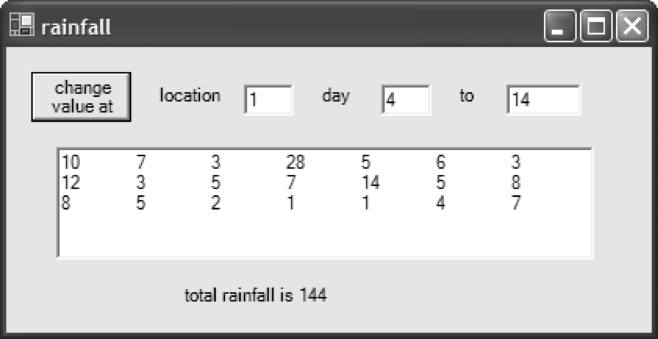
\includegraphics[width=10cm]{arrays-2d_rainfall_screen}
			\caption{The display from the rainfall program.}
			\label{fig:arrays-2d_rainfall_screen}
		\end{figure}

		First we declare the array:
		\begin{lstlisting}
Dim rainData(, ) As Integer =
	{{10, 7, 3, 28, 5, 6, 3},
	 {12, 3, 5, 7, 12, 5, 8},
	 { 8, 5, 2, 1, 1, 4, 7}}
		\end{lstlisting}
		To display all the data:
		\begin{lstlisting}
Private Sub Display()
	Dim location As Integer
	Dim dayNumber As Integer
	TextBox1.Clear()
	For location = 0 To 2
  		For dayNumber = 0 To 6
			TextBox1.AppendText(CStr(rainData(location, dayNumber))
				& Tab)
		Next
		TextBox1.AppendText(NewLine)
	Next
End Sub
		\end{lstlisting}
		The inner \keyword{For} loop deals with the different days, while the outer \keyword{For} loop deals with the different locations. The method uses the property \keyword{Tab}, which is in a library together with \keyword{NewLine} and can be used as shown provided that the following \keyword{Imports} statement is present at the head of the program:
		\begin{lstlisting}
Imports Microsoft.VisualBasic.ControlChars
		\end{lstlisting}
To change an element in the array, the day number, location number and new data value are extracted from their text boxes:
		\begin{lstlisting}
Private Sub ChangeValue()
	Dim dataValue As Integer
	Dim dayNumber As Integer
	Dim location As Integer
	dayNumber = CInt(DayTextBox.Text)
	location = CInt(LocationTextBox.Text)
	dataValue = CInt(ValueTextBox.Text)
	rainData(location, dayNumber) = dataValue
	Display()
	CalculateTotal()
End Sub
		\end{lstlisting}
		To calculate the total rainfall across all the locations:
		\begin{lstlisting}
Private Sub CalculateTotal()
	Dim location As Integer
	Dim dayNumber As Integer
	Dim total As Integer = 0
	For location = 0 To 2
		For dayNumber = 0 To 6
			total = total + RainData(location, dayNumber)
		Next
	Next
	Label1.Text = "total rainfall is " & total
End Sub
		\end{lstlisting}
		When you run this program, be careful to enter row numbers in the range 0 to 2, and column numbers in the range 0 to 6.
		
		You will see again that it is very common to see nested \keyword{For} statements used with two-dimensional arrays, because they make the maximum use of the uniformity of arrays.


	\section{\keyword{For Each} statement}
		The \keyword{For Each} statement can make loops more concise. Here, for example, is a method given above to calculate the total rainfall:
		\begin{lstlisting}
Private Sub CalculateTotal()
	Dim total As Integer = 0
	For Each item As Integer In rainData
		total = total + item
	Next
	TotalLabel.Text = "total rainfall is " & total
End Sub
		\end{lstlisting}
		In this version, there is no explicit mention of index values. At each repetition, the value of the variable \keyword{item} takes on the next value from the array.

	\section{Programming principles}
		A two-dimensional array is a collection of data, with a single name (for example \keyword{rainData}). An array can be visualized as a two-dimensional table, with rows and columns. Suppose we want to represent the rainfall data for each of seven days at each of three places. We declare an array:
		\begin{lstlisting}
Dim rainData(6, 2) As Integer
		\end{lstlisting}
		Elements in such an array are distinguished by specifying two indices, which are integers, for example \keyword{rainData(4, 2)}. You can think of the first index as describing the row number and the second as describing the column number. When the array is created the greatest value of the index of the array is specified - six and two in this example. This means that this array has seven rows and three columns. Indices always start at 0. In this example the row indices go from 0 to 6 and the column indices from 0 to 2.
		
		The elements of an array can be any type - \keyword{Integer}, \keyword{Double}, \keyword{String}, or any other object. But all the elements in an array must be of the same type - \keyword{Integer} in this example. The exception is when an array is declared to consist of \keyword{Object}. In this case such an array can accommodate any mix of objects.
		
		It is common to use nested \keyword{For} loops in conjunction with two-dimensional arrays.
		
		In this book we have explored both one-dimensional and two-dimensional arrays. VB provides for arrays with up to 60 dimensions, but dimensions above 3 are rarely used in practice.


	\section{Programming pitfalls}
		A common error in VB is to confuse the length of an array with the range of valid indices. For example, the array:
		\begin{lstlisting}
Dim table(10,5) As Integer
		\end{lstlisting}
		has 11 rows and 6 columns. The valid range of indices for the rows is 0 to 10. The valid range of indices for the columns is 0 to 5. Reference to \keyword{table(11, 6)} will give rise to the program stopping and an error message being displayed.


	\section{Summary}
		\begin{itemize}
      \item A two-dimensional array is a collection of data in a table, with rows and columns.
      \item An array is given a name by the programmer.
      \item An array is declared, along with other variables, like this:
				\begin{lstlisting}
Dim alice(24,30) As Integer
				\end{lstlisting}
				in which 24 is the greatest index of the rows and 30 is the greatest index of the columns.
      \item An individual element of an array is referred to by integer indices, for example:
				\begin{lstlisting}
alice(12, 3) = 45
				\end{lstlisting}
		\end{itemize}


	\section{Exercises}
		Basic operations on two-dimensional arrays
		\begin{EXE}
			\item	\name{Data handler} Write a program that uses a 4 x 7 array of numbers similar to the rainfall program (with output as shown in Figure 15.2). Extend the program to carry out the following methods:
				\begin{itemize}
		      \item When a button is pressed marked 'sums', add up the values for each of the seven columns and add up all the values of each of the four rows and display them.
     			\item When a button marked 'largest' is pressed, find the largest value in each row, the largest in each column and the largest value in the complete array.
			    \item When a button marked 'scale' is pressed, multiply every number in the array by a number entered into a text box. (This could be used to convert from centimetres to inches.)
				\end{itemize}
		\end{EXE}
			
		Statistical measures
		\begin{EXE}
			\item	Extend the rainfall program so that it provides a button to calculate the average rainfall per day for each location. So for example the average rainfall per day in location two might be 23.
				
			Extend it further to provide a button to calculate the mean and standard deviation of the daily rainfall in any location. So for illustration, the mean rainfall in any location could be 19, with a standard deviation of 6.4.
		\end{EXE}
			
		Bar charts and pie charts
		\begin{EXE}
		\item	Extend the rainfall program so that the user can specify a row (a location). 
				
			The information is then displayed as a bar chart.
				
			Extend the program to display the information in a single row or a single column as a pie chart.
		\end{EXE}
			
		Mathematical operations
		\begin{EXE}
			\item	\name{Transpose} The transpose of an array is the technical term used to describe swapping the elements in an array across one of the diagonals. The numbers on the diagonal do not change. So if an array is:
				\begin{center}
					\begin{tabular}{|c|c|c|c|}
						\hline
						1 & 2 & 3 & 4 \\ \hline
						5 & 6 & 7 & 8 \\ \hline
						9 & 10 & 11 & 12 \\ \hline
						13 & 14 & 15 & 16 \\ \hline
					\end{tabular}
				\end{center}

				then its transpose is:
				\begin{center}
					\begin{tabular}{|c|c|c|c|}
						\hline
						1 & 5 & 9 & 13 \\ \hline
						2 & 6 & 10 & 14 \\ \hline
						3 & 7 & 11 & 15 \\ \hline
						4 & 8 & 12 & 16\\ \hline
					\end{tabular}
				\end{center}

				Write a program to input the elements of an array in the same manner as the rainfall program. It transposes the array when a button is pressed, and displays it.
		\end{EXE}

		Games
		\begin{EXE}
			\item	\name{Tic tac toe} Tic tac toe (or noughts and crosses) is played on a 3 × 3 grid, which is initially empty. Each of two players goes in turn. One places a cross in a blank square the other places a nought in a blank square.
				
		 		The winner is the person who gets a line of three noughts or three crosses. 
			
				Thus a win for noughts might look like this:
				\begin{center}
					\begin{tabular}{c|c|c}
						o & x & o \\ \hline
						x & o & \\ \hline
						x &  	& o 
					\end{tabular}
				\end{center}

				Games can end in a draw, where neither side has obtained a line.
				
				Write a program to play the game. There is just one button to start a new game. The program shows the noughts and crosses graphically, each in its own picture box. The human player specifies a move by clicking with the mouse on the picture box where the cross is to be placed. The other player is the computer, which plays as noughts and decides where to play on a random basis.
		\end{EXE}

		Artificial life
		\begin{EXE}
			\item \name{Cellular life} An organism consists of single cells that are on (alive) or off (dead). Each generation of life consists of a single row of cells. Each generation of life (each row) of the organism depends on the previous one (just like real life). Time moves downwards, from top to bottom. Each row represents a generation. The lives look like this:
				\begin{center}
					\begin{tabular}{|c|c|c|c|c|c|c|c|c|c|c|}
						\hline
						& 	& 	& 	& 	& * & 	& 	& 	& 	& \\ \hline
						& 	& 	& 	& *	& *	& * & 	& 	& 	& \\ \hline
						& 	& 	& * & *	&		& 	& * & 	& 	& \\ \hline
						& 	& *	& *	&	 	& * &	*	& *	& * & 	& \\ \hline
						&	*	& *	&		&   & *	&		&	 	& 	& * & \\ \hline
					*	& *	&	  & *	& * &	*	& *	&	  & *	& *	& *\\ \hline
					\end{tabular}
				\end{center}
				In the beginning, there is just one cell alive. Whether a cell is alive or dead depends on a combination of factors - whether or not it was alive in the last generation and whether or not its immediate neighbours were alive in the last generation. You can see that, even after only five generations, a pattern is emerging. These patterns are very subtle and mimic the patterns found in real living organisms. The rules are as follows.
				A cell lives only if:
				\begin{itemize}
		      \item it was dead, but only its left neighbour was alive;
     			\item it was dead, but only its right neighbour was alive;
		      \item it was alive, but its immediate neighbours were dead;
		      \item it was alive, and only its right neighbour was alive.
				\end{itemize}
				So, for example, given the following generation:
				\begin{center}
					\begin{tabular}{|c|c|c|c|c|}
						\hline
							& *	& *	& *	& \\ \hline
					\end{tabular}
				\end{center}

				\begin{itemize}
		      \item The first cell lives, because even though it was dead, its immediate right neighbour was alive.
		      \item The second cell lives because only its immediate right neighbour was alive.
		      \item The third living cell dies (through overcrowding, we surmise!).
		      \item The fourth cell dies.
     			\item The fifth cell lives because, although it was dead, its immediate left neighbour was alive.
				\end{itemize}
				So the new generation is:
				\begin{center}
					\begin{tabular}{|c|c|c|c|c|}
						\hline
						*	& *	& & & *	\\ \hline
					\end{tabular}
				\end{center}

				Write a program that uses a two-dimensional array to chart the progress of the life form. Display the development on the screen as asterisks, as above. Provide a button that allows the user to go on to the next generation.
			\item	\name{Conway's Game of Life} In this life form, again, an organism consists of single cells that are on (alive) or off (dead). The organisms exist in a two-dimensional grid world, for example:

		\begin{center}
					\begin{tabular}{|c|c|c|c|c|c|c|c|}
						\hline
						& 	& 	& 	& 	&  	& 	&  \\ \hline
						& 	& *	& 	& *	&  	& 	&  \\ \hline
						& *	& 	& *	& *	&  	& 	&  \\ \hline
						& 	& 	& *	& 	& * & 	& \\ \hline
						& 	& *	& 	& 	&  	& 	&  \\ \hline
						& 	&   & 	& 	&  	& 	&  \\ \hline
						& *	& 	& 	& 	&  	& 	&  \\ \hline
						& 	& 	& 	& 	&  	& 	&  \\ \hline
					\end{tabular}
				\end{center}
				The rules governing this organism are:
				\begin{itemize}
     			\item If a live cell has two or three neighbours, it will survive. Otherwise it will die of isolation or overcrowding.
		      \item If an empty cell is surrounded by exactly three cells, then a new live cell will be born to fill the space.
     			\item All births and deaths take place simultaneously.
				\end{itemize}
				Write a program to simulate this kind of life. The program should initially allow the user to click on the cells that are to be alive. Provide a button that allows the user to go on to the next generation and display it.
					
				The program needs two arrays - one to represent the current state of life and another to represent the next generation. After each new generation is created, the roles of the two arrays are swapped.
		\end{EXE}


		\begin{stab}
			\begin{enumChapter}
				\item	Column 5 is Saturday. 31 computers were sold at shop 3 on Thursday. This is row 3 and column 3.
				\item
					\begin{lstlisting}
Dim chessBoard(7, 7) As String
					\end{lstlisting}
				\item	
					\begin{lstlisting}
Dim chessBoard(7, 7) As String
Dim row, col As Integer
For row = 0 To 7
	For col = 0 To 7
		chessBoard(row, col) = "empty"
	Next
Next
					\end{lstlisting}
				\item	The largest index is 7.
				\item
					\begin{lstlisting}
Dim numbers(,) As String = { 
	{"one", "two", "three"},
	{"four", "five", "six"},	
	{"seven", "eight", "nine"}
}
					\end{lstlisting}
			\end{enumChapter}
		\end{stab}
